%%%%%%%%%%%%%%%%%%%%%%%%%%%%%%%%%%%%% 
% Check out the accompanying book, Even Better Books with LaTeX the Agile Way in 2023, for a discussion of the template and step-by-step instructions. https://amzn.to/3HqwgXM https://leanpub.com/eBBwLtAW/
% The template was originally created by Clemens Lode, LODE Publishing (www.lode.de), on 1/1/2023. Feel free to use this template for your book project! 
% I would be happy if you included a short mention in your book in order to help others to create their own books, too ("Book template based on \textit{Even Better Books with LaTeX the Agile Way in 2023} by Clemens Lode").
% Contact me at mail@lode.de if you need help with the template or are interested in our editing and publishing services.
% And don't forget to follow us on Instagram! https://www.instagram.com/lodepublishing/ https://www.instagram.com/betterbookswithlatex/
%%%%%%%%%%%%%%%%%%%%%%%%%%%%%%%%%%%%%

%%%%%%%%%%%%%%%%%
% This is an excerpt from the accompanying book, Even Better Books with LaTeX the Agile Way in 2023. https://www.amazon.com/Better-Books-LaTeX-Agile-Book-ebook/dp/B0BMZJ5LF7
%%%%%%%%%%%%%%%%%


\chapter{Generate Your First E-book}\label{generateyourfirstebook:cha}

\textit{So\dots{} how do we use LaTeX? What do we need to install, set up, etc.? And just how do we use LaTeX to create an e-book?} For now, we will focus on getting you started generating a PDF and e-book. Later, in Chapter~\ref{fillingthetemplate:cha}, we will go step by step through the process of copying your book from your text source (e.g., Word) to the template.

\section{LaTeX Support}\label{latexhelp:sec}

While we have tested the template that comes with this book several times, you will likely encounter an issue not discussed here. Creating a document in LaTeX \textit{is} more complex than doing so in Word, but even in Word, there are issues you might run into where the solution is not immediately apparent.\index{LaTeX@\textit{LaTeX}!support} 

If you encounter any error or have a question about LaTeX as it is used in the template, please do not hesitate to contact us. The question and the answer might be added to an FAQ for other readers. We offer free support if you provide us with a link to your Overleaf project. For major changes, one of our LaTeX developers can help you at an affordable rate. But most issues can probably be solved immediately and at no cost (``You forgot to close the parentheses,'' ``You need to load package X,'' ``Your graphics file is corrupt,'' etc.). Simply contact us at \textbf{mail@lode.de} and we will see what we can do!

For general LaTeX questions, you can also check out the community at \url{https://tex.stackexchange.com}.\index{LaTeX@\textit{LaTeX}!support!community} If you post a brief (but working) example with LaTeX code with which you are having a problem, the community can usually provide high-quality advice. If you encounter specific technical issues with the tex4ebook, you can also check whether there are open issues on the website of the tex4ebook maintainer: \url{https://github.com/michal-h21/tex4ebook}.


\section{Signing up at Overleaf}

Before we start, yes, setting up LaTeX the first time is more complicated than writing a letter in Word. But there are many solutions available that allow you to use LaTeX without much hassle. One of those solutions is Overleaf\index{Overleaf@\textit{Overleaf}}, which I am using for writing this very book (and all my other books). Overleaf is a collaborative online editor and project manager for LaTeX documents. It is available free for smaller projects that do not require password protection. If you want to keep your LaTeX code private, I recommend the Pro upgrade, which also adds full project history, access management, priority support, and support for larger projects. 

\textit{If your goal is to try things out and work on your book with a professional editor, you do not have to spend money on Overleaf for private projects or larger projects. We can host the project on our Overleaf account and manage everything for you. Drop us a message at mail@lode.de!}

\babelEN{\begin{definition}{Overleaf} \textit{Overleaf} is an online editor and project manager for LaTeX documents. It manages your project with a versioning system and automatically compiles your LaTeX code into PDF and (with some help) HTML. It is free for public projects and does not require installation or setup. You can get an account here: \url{https://www.overleaf.com}.\end{definition}}\index{Overleaf@\textit{Overleaf}|textbf}


Overleaf requires no installation.\index{Overleaf@\textit{Overleaf}!features} Just register an account, use my template, fill in your text, and you are ready to download the necessary files for creating a print book or e-book. If you are using a different LaTeX website or your own local installation, a different configuration might be required.\index{Overleaf@\textit{Overleaf}!register}\index{Overleaf@\textit{Overleaf}!sign up} To register an account on Overleaf\index{Overleaf@\textit{Overleaf}}, simply go to \url{https://www.overleaf.com}, enter your email and password, confirm the email, and log into your Overleaf account at \url{https://www.overleaf.com} clicking on \textbf{Log In}.


\section{Copy the Template}\label{copytemplate:sec}

\textit{If you do not want to use the template, check out the appendix of the accompanying book, (\textit{Even Better Books with LaTeX the Agile Way in 2023: Streamline Your Writing Process and Connect with Readers from Day One}, \url{https://amzn.to/3GCEGen}).}


Once you have your account, you have two options to get the template:

\begin{itemize}
\item go to \url{https://tinyurl.com/latextemplate2023}; or 
\item go to \url{https://www.overleaf.com/latex/templates}, searching for \textbf{Book Template for Amazon KDP, Leanpub, and Google Play (e-book and PDF) 2023}\index{template! copying}, clicking on the entry, and pressing \textbf{Open as Template}. Note that there is an earlier version available as well. Make sure you get the 2023 version!\index{template}
\end{itemize}

Once copied, you can access the template via your Overleaf project view (go to \url{https://www.overleaf.com} and click on \textbf{Projects}\index{Overleaf@\textit{Overleaf}!template} or go directly to \url{https://www.overleaf.com/project}); your new project should be listed there. 

The template itself needs to be adapted, of course\emdash{}after all, it is \textit{your} book, not mine. But for now, let us focus first on how to get from the template to a book. 

So, navigate to your project view (\url{https://www.overleaf.com}, \textbf{Projects}) and click on the new project \textbf{Book Template for Amazon KDP, Leanpub, and Google Play (e-book and PDF) 2023}. In the opened window, you should see a menu bar at the top with the \textbf{Menu} button that opens the options for the project. On the right, you will see a preview of the PDF output. Remember what I mentioned at the beginning of the book: LaTeX is not a ``what you see is what you get'' editor. Instead, whatever you write has to be compiled into a PDF. Hence, you have the actual editing window in the middle (horizontally) and the separate output window on the right side of the screen.

\begin{figure}[H]\centering
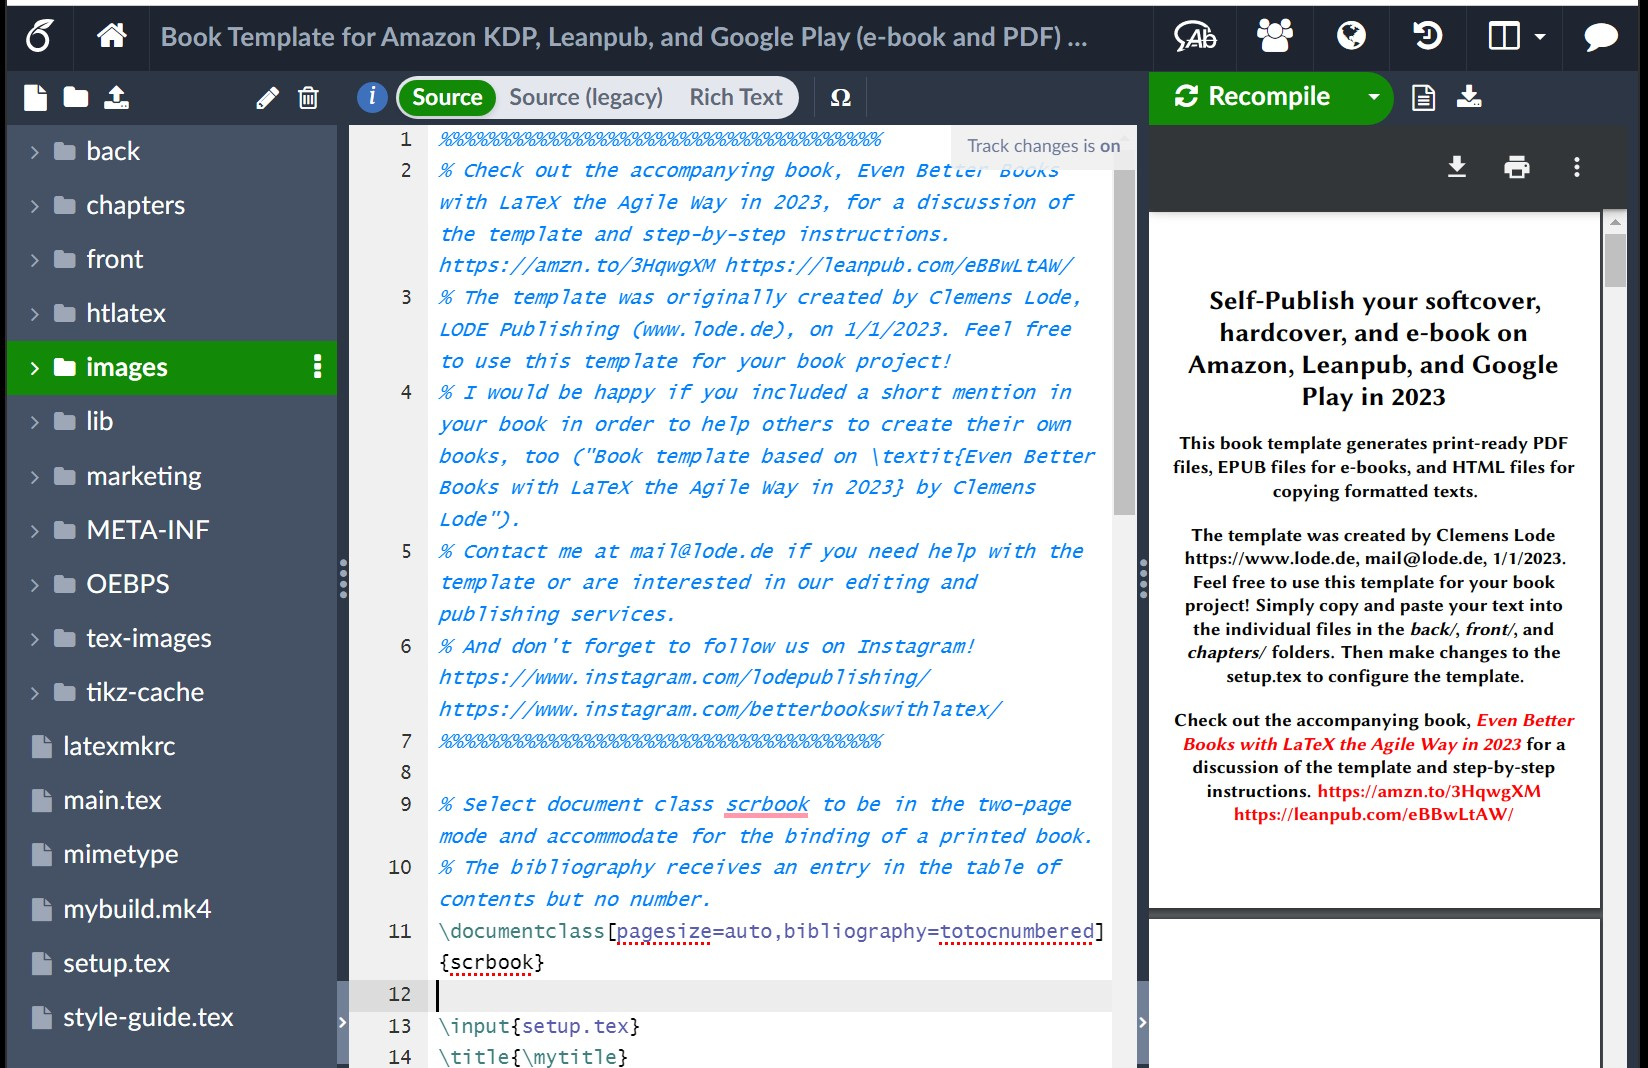
\includegraphics[width=\textwidth]{images/overleaf.jpg}
\caption{The project screen in Overleaf.}
\label{overleaf:fig}
\end{figure}



\section{Create a PDF}\label{createpdfoutput:sec}

The template is set up to produce both EPUB and PDF files.\index{template!EPUB output} The EPUB files can later be converted into formats that can be read by a Kindle e-book reader, while the PDF files can be used for printing or reading on a computer screen. In addition, there is an option to turn your LaTeX project into a HTML file to be used for easy copy and paste. For now, let us first create a PDF.\index{PDF!create}\index{create PDF}

Click on the \textbf{Menu} button at the top left. A new panel shows up (see Figure~\ref{projectsettings:fig}). In the \textbf{Settings} section, click on the drop-down menu right of \textbf{Compiler}. We want the PDF output\index{PDF!output}, so select \textbf{XeLaTeX} and select \textbf{2022} as the \textbf{TeX Live version}.

\begin{figure}[H]\centering
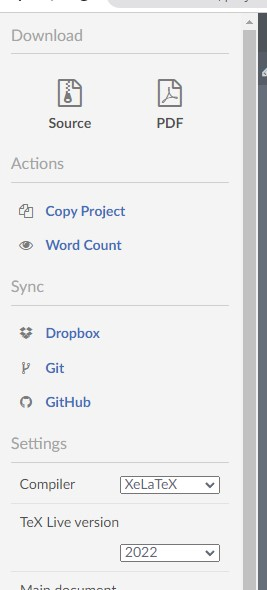
\includegraphics[width=0.4\textwidth]{images/projectsettings.jpg}
\caption{The project settings screen in Overleaf.}
\label{projectsettings:fig}
\end{figure}

\begin{definition}{XeLaTeX} \textit{XeLaTeX} is a LaTeX typesetting engine with an extended font, as well as UTF-8 encoding (for special characters) support. It takes longer to compile with \textit{XeLaTeX} than with the more basic \textit{pdfLaTeX}.\end{definition}\index{XeLaTeX@\textit{XeLaTeX}|textbf}





To download the PDF\index{PDF!download} of the \textit{XeLaTeX} output, simply click on the third symbol (\textbf{Download PDF}, the second symbol to the right of \textbf{Recompile} in the PDF view, see Figure~\ref{downloadpdf:fig}).


\begin{figure}[H]\centering
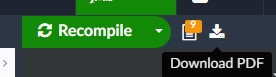
\includegraphics[width=0.4\textwidth]{images/downloadPDF.jpg}
\caption{Download the PDF via the PDF view.}
\label{downloadpdf:fig}
\end{figure}


Alternatively, you can click on \textbf{Menu} on the top left and click on \textbf{PDF} (see Figure~\ref{downloadpdfmenu:fig}).

\begin{figure}[H]\centering
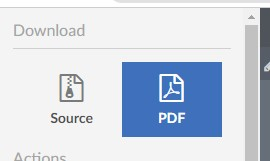
\includegraphics[width=0.4\textwidth]{images/downloadPDF2.jpg}
\caption{Download the PDF via the Menu.}
\label{downloadpdfmenu:fig}
\end{figure}

Done! Your first PDF. This PDF could be used to upload to on-demand book services like Amazon's KDP.


\section{Create the EPUB Output}\label{createhtmlloutput:sec}

To create the EPUB file, we need to switch from \textit{XeLaTeX} to \textit{pdfLaTeX} output.\index{PDF!switch to EPUB output}\index{EPUB!switch to PDF output} For this, click on the \textbf{Menu} button at the top left, and this time, select \textit{pdfLaTeX} in the \textbf{Settings} section, in the drop-down menu to the right of \textbf{Compiler} (see Figure~\ref{switchpdflatex:fig}).

\begin{definition}{pdfLaTeX} \textit{pdfLaTeX} is a basic LaTeX typesetting engine that translates LaTeX documents directly into PDFs or HTML files (with the help of \textit{TeX4ht}).\end{definition}\index{pdfLaTeX@\textit{pdfLaTeX}|textbf}

\begin{figure}[H]\centering
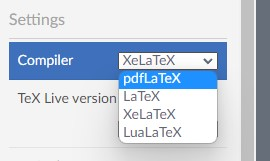
\includegraphics[width=0.4\textwidth]{images/switchpdflatex.jpg}
\caption{Switch to EPUB generation by changing the compiler in the Menu to pdfLaTeX.}
\label{switchpdflatex:fig}
\end{figure}

Next, on the left side, scroll down to \textit{latexmkrc} (see Figure~\ref{latexmkrc:fig}).

\begin{figure}[H]\centering
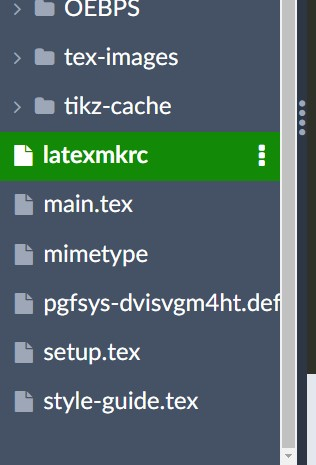
\includegraphics[width=0.4\textwidth]{images/latexmkrc.jpg}
\caption{Click here to select the \textit{latexmkrc} file.}
\label{latexmkrc:fig}
\end{figure}

There, remove the ``\#'' in front of this line (first option):

\begin{lstlisting}
# system("tex4ebook -j output -c htlatex/enumerate-fix main");
\end{lstlisting}

If you are switching back to XeLaTeX, remember to comment out this line again (add a ``\#'').

Switching the output requires you also to recompile your project. For this, click on \textbf{Recompile} in the menu above the preview window on the right (see Figure~\ref{recompile:fig}).


\begin{figure}[H]\centering

\includegraphics[width=0.4\textwidth]{images/recompile.jpg}
\caption{Click here to recompile the project.}
\label{recompile:fig}
\end{figure}

Before continuing, wait until the compilation is finished. If you encounter a problem here (and a little red box with a number appears on the document icon right beside \textbf{Recompile}, see Figure~\ref{error:fig}), please contact me at \textbf{mail@lode.de} and I will help you as soon as possible to fix the issue.\index{recompile}\index{refresh} A possible fix (especially after switching compilers) is clicking on ``Logs and output files'', then on the red \textbf{Clear cached files} button, and then again on \textbf{Recompile}.

\begin{figure}[H]\centering
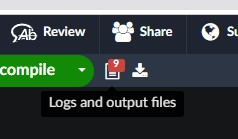
\includegraphics[width=0.4\textwidth]{images/error.jpg}
\caption{A red box with a number on the document icon indicates an error.}
\label{error:fig}
\end{figure}

If no number appears or if there are only warnings (orange box), you can proceed with the download.\index{error!compilation}\index{recompile} 

\section{Download and Convert EPUB to Kindle}\label{converthtmltokindle:sec}
\index{EPUB!convert to Kindle}

We need another tool to publish the e-book on Amazon, namely the \textit{Kindle Previewer}.\index{Kindle Previewer@\textit{Kindle Previewer}} Go to \url{https://www.amazon.com/Kindle-Previewer/b?node=21381691011} and scroll down to the download links. If the link is unavailable or broken, simply search for \textbf{Amazon Kindle Previewer} using a search engine. Once downloaded, start the installation. It will associate EPUB files with Kindle Previewer, meaning you need only to download the EPUB files to convert them.

\babelEN{\begin{definition}{Kindle Previewer} \textit{Kindle Previewer} is a Windows and MAC tool to load HTML and EPUB files and convert them into KPF and MOBI files for upload to Amazon. The tool also allows you to preview the file as a customer would see it on a Kindle eReader.\end{definition}}\index{Kindle Previewer|textbf}

For downloading the e-book,\index{template!e-book!downloading} you have to download the \textbf{EPUB} file by clicking on the \textbf{Logs and output files} icon at the top of the right window, scrolling all the way down to \textbf{Other logs \& files}, and selecting the \textbf{output.epub} entry, see Figure~\ref{downloadepub:fig}).\index{EPUB!download} 

\begin{figure}[H]\centering
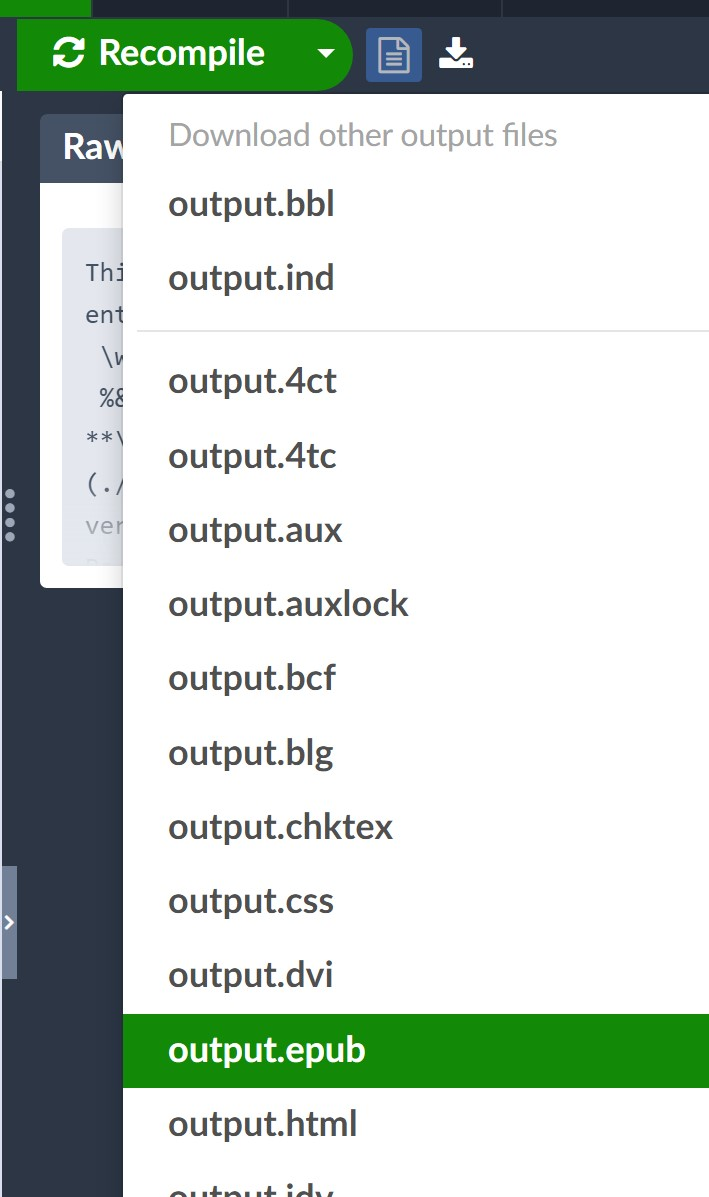
\includegraphics[width=0.65\textwidth]{images/downloadEPUB.jpg}
\caption{The EPUB file with the HTML output, style information, and images can be downloaded in the ``Logs and output files'' screen at the very bottom.}
\label{downloadepub:fig}
\end{figure}

A download with the EPUB file should start now, and, once completed, Kindle Previewer should start automatically (or you first need to click on the file, depending on your browser's configuration). If you want to convert an EPUB file already downloaded on your computer, start the Kindle Previewer manually, select \textbf{File / Open Book} (see Figure~\ref{kindlepreviewer:fig}), browse to the directory where you have the EPUB file, and press \textbf{Open}. This starts the conversion process.

\begin{figure}[H]\centering
\adjustbox{max height=.35\textheight}{
    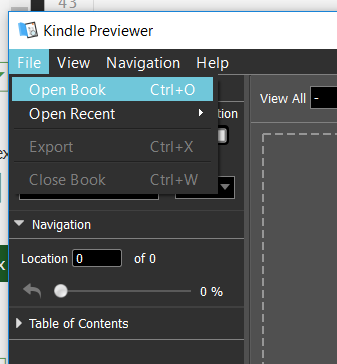
\includegraphics{images/kindlepreviewer.png}
}
\caption{Importing the EPUB file in Kindle Previewer to convert it into a KPF or MOBI format.}
\label{kindlepreviewer:fig}
\end{figure}

Note that if you also want the HTML output (for example, to copy contents), check out the appendix of the accompanying book, (\textit{Even Better Books with LaTeX the Agile Way in 2023: Streamline Your Writing Process and Connect with Readers from Day One}, \url{https://amzn.to/3GCEGen}).


\section{Converting EPUB to KPF with the Kindle Previewer}

\textit{For general information about the Kindle Previewer, check out its homepage at \url{https://kdp.amazon.com/en_US/help/topic/G202131170}}

Depending on the book size, converting an EPUB file to a KPF file might take a moment. During conversion, you will see the ``Converting your book to Kindle format'' message on the screen. Once finished, a virtual Kindle reader\index{Kindle!preview} should show up where you can browse through your book. If you are happy with how the contents look, press \textbf{File / Export} in the menu, and press \textbf{Export}. For the name of the exported file, I recommend including the current date to prevent confusion when uploading (for example, \textit{ebbwltaw-01012023.kpf}). You can select different output formats. Choose the (pre-selected) format \textbf{Books(.kpf)}, which is the newest and most compatible format.

A message box should appear that reads ``Book is successfully exported here.'' You can safely ignore the warning message ``Enhanced typesetting is enabled for the book being previewed, but it is not supported in the exported file.'' This refers only to the fact that any fonts you are using in your LaTeX project are ignored and replaced by the respective fonts of the e-book reading device. Now you have a KPF file\index{KPF!convert from EPUB} that you can use later to upload to Amazon's KDP platform and release it directly as an e-book on Amazon. I discuss the details in the accompanying book, (\textit{Even Better Books with LaTeX the Agile Way in 2023: Streamline Your Writing Process and Connect with Readers from Day One}, \url{https://amzn.to/3GCEGen}), but in essence, that is the entire publishing process, at least from the technical side.



\section{Versioning}\label{versioning:sec} \index{versioning}

\textbf{Before you continue:} while you are learning LaTeX, you should create a backup\index{backup!create}\index{Overleaf@\textit{Overleaf}!backup} whenever your project compiles successfully. You can click on \textbf{History} (top menu, see Figure~\ref{versions:fig}), then on \textbf{All history}, then on \textbf{View single version}, then on \textbf{Label this version}, then enter a name for the backup.

\begin{figure}[H]\centering
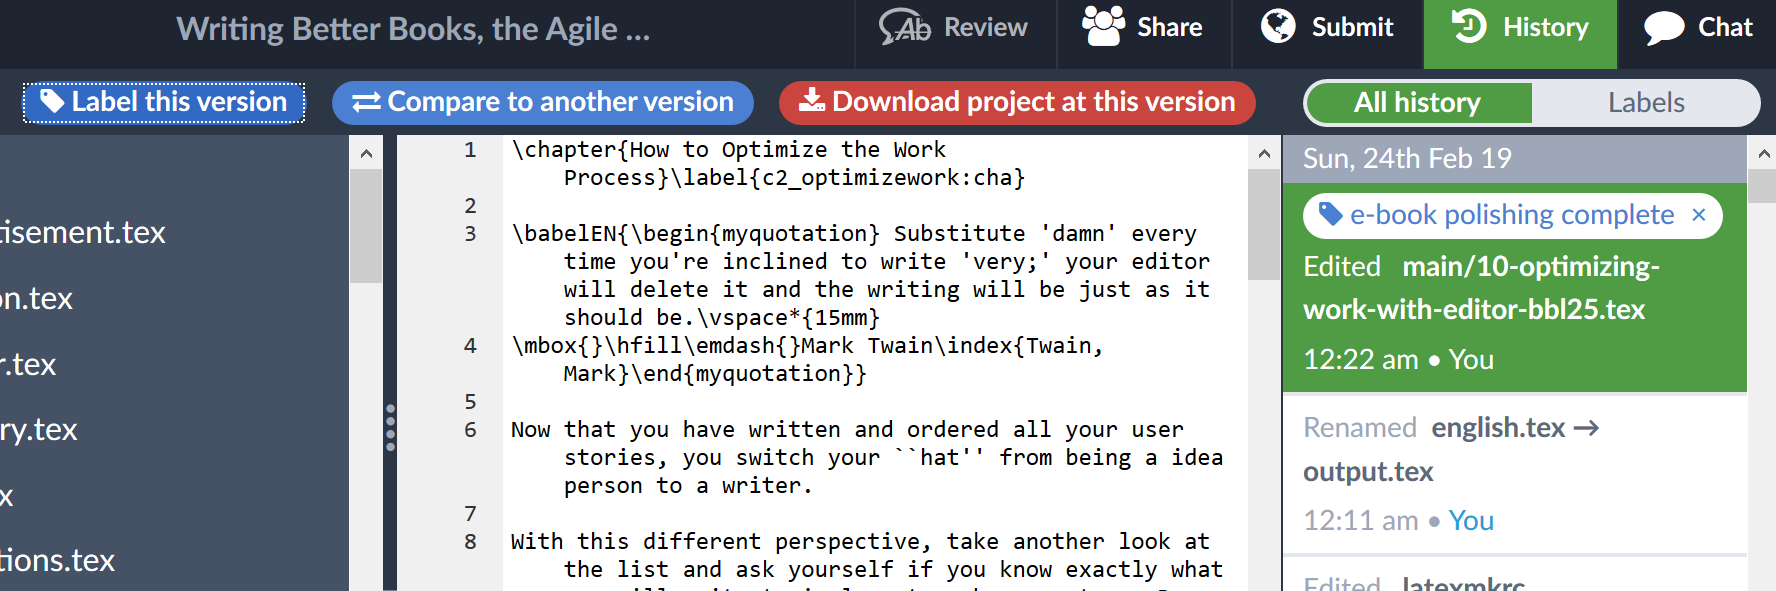
\includegraphics[width=0.95\textwidth]{images/versions.png}
\caption{Setting the name of the current version of the book for later reference.}
\label{versions:fig}
\end{figure}

It is best to name each backup\index{backup!naming} by the milestone you have reached so that you later know at what point you have made the backup. For example, after polishing the files for an e-book release (but before polishing it for print), you could name it ``e-book polishing complete.''

You can always go back to a previous version and compare your changes. Click on \textbf{History}, then on \textbf{Compare to another version}, then on \textbf{Labels}, and then on a file in the list on the left side with a note ``edited'' right beside it. That being said, you do not have to save as you write. Your latest changes are always saved automatically. 

\textbf{Summary:} This chapter showed you how to generate a PDF file and an EPUB file from the LaTeX template. You signed up at Overleaf, copied the template, switched the output from XeLaTeX to pdfLaTeX, downloaded the PDF and EPUB files, converted the EPUB to KPF with the Kindle Previewer, and created backups of your project.